\documentclass[11pt,a4paper]{article}
\usepackage[margin=2.6cm]{geometry}
\usepackage{amsmath,amssymb,amsthm}
\usepackage{booktabs}
\usepackage{graphicx}
\usepackage{caption}
\usepackage{subcaption}
\usepackage[numbers,sort&compress]{natbib}
\usepackage{microtype}
\usepackage{xcolor}
\usepackage[colorlinks=true,linkcolor=blue!60!black,citecolor=blue!60!black,urlcolor=blue!60!black]{hyperref}
\usepackage{mathptmx}
\usepackage{listings}
\captionsetup{font=small,labelfont=bf}
\emergencystretch=1.5em

% Float placement. With six figures and seven tables in fourteen pages of text,
% the default LaTeX float parameters queue floats until they spill past the
% bibliography. Loosening the page fractions and adding a barrier at each
% section keeps every float inside the section that discusses it.
\usepackage[section]{placeins}
\renewcommand{\topfraction}{0.9}
\renewcommand{\bottomfraction}{0.8}
\renewcommand{\textfraction}{0.07}
\renewcommand{\floatpagefraction}{0.75}
\setcounter{topnumber}{3}
\setcounter{bottomnumber}{2}
\setcounter{totalnumber}{4}
\graphicspath{{figures/}}

% Every table, every figure and every number quoted in the running text is
% generated from the census by code/run_all.py; none of them are stored in this
% repository. That is deliberate: the manuscript cannot then disagree with the
% computation. If the generated files are absent, stop here with an actionable
% message rather than with a pile of "undefined control sequence" errors.
\IfFileExists{tables/macros.tex}{}{%
  \PackageError{fgp}{%
    ^^J
    ================================================================^^J
    The generated tables, figures and numbers are missing.^^J
    ^^J
    Build them first, from the repository root:^^J
    ^^J
    \space\space\space\space make^^J
    ^^J
    or, without make:^^J
    ^^J
    \space\space\space\space python3 code/run_all.py data/fgp_layers.csv --out paper^^J
    ^^J
    See README.md for the full sequence, including building the census.^^J
    ================================================================^^J
  }{Run the pipeline, then build the manuscript again.}%
}
\newcommand{\nScales}{20}
\newcommand{\Nfirst}{200\,000}
\newcommand{\Nlast}{455\,052\,511}
\newcommand{\Xfirst}{2\,750\,159}
\newcommand{\Xlast}{9\,999\,999\,967}
\newcommand{\CfitFirst}{1.2483}
\newcommand{\CfitLast}{1.1460}
\newcommand{\CWFirst}{1.0783}
\newcommand{\CWLast}{1.0478}
\newcommand{\deltaFirst}{0.1700}
\newcommand{\deltaLast}{0.0982}
\newcommand{\spreadMin}{0.206}
\newcommand{\spreadMax}{0.352}
\newcommand{\netChangePrimary}{0.102}
\newcommand{\nMonoDec}{20}
\newcommand{\nMonoInc}{0}
\newcommand{\envNineMin}{0.9999}
\newcommand{\envNineMax}{1.2709}
\newcommand{\narrowLast}{0.9999}
\newcommand{\envMaxLast}{1.2150}
\newcommand{\EtwoFirst}{0.84606}
\newcommand{\EtwoLast}{0.88815}
\newcommand{\EthreeFirst}{0.68323}
\newcommand{\EthreeLast}{0.76691}
\newcommand{\DFirst}{0.05643}
\newcommand{\DLast}{0.04505}
\newcommand{\DmidFirst}{0.10569}
\newcommand{\DmidLast}{0.08102}
\newcommand{\ratioMin}{0.99959}
\newcommand{\ratioMax}{1.00020}
\newcommand{\betaEtwo}{0.810}
\newcommand{\betaEtwoSE}{0.011}
\newcommand{\betaEthree}{0.782}
\newcommand{\betaEthreeSE}{0.012}
\newcommand{\betaD}{0.592}
\newcommand{\betaDSE}{0.017}
\newcommand{\EtwoAtFifty}{0.059}
\newcommand{\EtwoAtTwoHundred}{0.019}
\newcommand{\zEtwoEnd}{21}
\newcommand{\zEthreeEnd}{16}
\newcommand{\zDEnd}{10}
\newcommand{\medzEtwo}{4.5}
\newcommand{\medzEthree}{3.7}
\newcommand{\medzD}{2.8}
\newcommand{\towardEtwo}{17}
\newcommand{\towardEthree}{17}
\newcommand{\towardD}{17}
\newcommand{\nSteps}{18}
\newcommand{\zFirstStepEtwo}{-0.12}
\newcommand{\zFirstStepEthree}{-0.20}
\newcommand{\zFirstStepD}{-0.89}
\newcommand{\gstarFirst}{14.13}
\newcommand{\gstarLast}{22.37}
\newcommand{\ratioMean}{0.962}
\newcommand{\ratioSD}{0.011}
\newcommand{\deficitFirst}{0.69}
\newcommand{\deficitLast}{0.66}
\newcommand{\bandSpreadMax}{1.03}
\newcommand{\ratioAllMin}{0.913}
\newcommand{\ratioAllMax}{0.986}
\newcommand{\deficitMin}{0.48}
\newcommand{\deficitMax}{1.06}
\newcommand{\deficitMean}{0.69}
\newcommand{\deficitSD}{0.15}
\newcommand{\gstarLastSE}{0.27}
\newcommand{\deficitLastSE}{0.27}
\newcommand{\deficitLastVal}{0.66}
\newcommand{\ratioLastVal}{0.9715}
\newcommand{\ratioLastSE}{0.0116}
\newcommand{\sigmaUnity}{2.5}
\newcommand{\sigmaModel}{3.2}
\newcommand{\modelDeficitTen}{1.7149}
\newcommand{\modelDeficitHundred}{1.5167}
\newcommand{\richardson}{1.4992}
\newcommand{\verifyLayers}{1\,544}
\newcommand{\verifyMismatch}{0}
\newcommand{\verifyXmax}{2\,038\,074\,743}
\newcommand{\verifySeconds}{20}
\newcommand{\sieveSeconds}{14}
\newcommand{\nSpecs}{36}
\newcommand{\sFirst}{1.1577}
\newcommand{\sLast}{1.0937}
\newcommand{\ampRatio}{1.28}
\newcommand{\ampRatioSD}{0.04}
\newcommand{\ampRatioMin}{1.20}
\newcommand{\ampRatioMax}{1.39}
\newcommand{\ampRatioPi}{1.12}
\newcommand{\ampRatioPiSD}{0.04}
\newcommand{\ampSlopeData}{0.78}
\newcommand{\ampSlopeModel}{0.62}
\newcommand{\wolfX}{325\,619\,971}
\newcommand{\wolfPublished}{1.187}
\newcommand{\wolfOurs}{1.1114}
\newcommand{\wolfEnvMin}{0.9382}
\newcommand{\wolfEnvMax}{1.1910}
\newcommand{\wolfInside}{inside}
\newcommand{\wolfBestC}{6}
\newcommand{\wolfBestGmin}{2}
\newcommand{\wolfBestEst}{unweighted least squares}
\newcommand{\wolfBestS}{1.1869}


\newtheorem{theorem}{Theorem}
\newtheorem{lemma}[theorem]{Lemma}
\newtheorem{proposition}[theorem]{Proposition}
\theoremstyle{remark}
\newtheorem{remark}[theorem]{Remark}

\newcommand{\Cfit}{C_{\mathrm{fit}}}
\newcommand{\CW}{C_W}
\newcommand{\logX}{\log X}
\newcommand{\Xeff}{X_{\mathrm{eff}}}
\newcommand{\Etwo}{E_2}
\newcommand{\Ethree}{E_3}
\DeclareMathOperator{\li}{li}

\title{Forward-Gap Layers of Consecutive Primes:\\
Window-Free Diagnostics of the Gallagher Limit\\
and a Derived Spatial Crossover at $g \approx \log X$}
\author{
Kamal Hassan$^{1}$ \qquad Farah Aymen$^{1}$\\[3pt]
\small $^{1}$The British University in Egypt, El Sherouk City, Cairo, Egypt\\
\small \texttt{kamal.hassan@bue.edu.eg}
\quad
\texttt{farah.aymen@bue.edu.eg}
}
\date{}

\begin{document}
\maketitle

\begin{abstract}
The frequency of a gap $g$ between consecutive primes below $X$ is expected, on the Hardy--Littlewood conjectures, to decay as $\exp(-g/\logX)$ once the arithmetic factor $H(g)$ is removed, with rescaled rate exactly $1$ in the limit (Gallagher). Computations since Brent (1974) have instead fitted a rate near $1.2$, and whether this reflects a constant or a slowly decaying finite-$X$ effect has remained open. We revisit the question with a complete census of consecutive prime gaps at \nScales{} log-spaced scales from $N=\Nfirst$ to $N=\pi(10^{10})=\Nlast$, organised by the forward gap of each prime, produced in \sieveSeconds{} seconds by released code and reproduced exactly by an independent implementation to $\verifyXmax$.

We first show that the fitted rate is not a function of $X$ alone: across \nSpecs{} defensible fitting specifications its value at a single scale spans $\spreadMin$ to $\spreadMax$, more than the total change of $\netChangePrimary$ over four decades of $X$ under any one specification. The one published value we could trace to a stated fitting procedure, Wolf's $s=\wolfPublished$ near $X=\wolfX$, is reproduced from our own census to four decimal places by changing the specification alone. We therefore replace the fitted rate with statistics that involve no window. Differencing consecutive census snapshots gives the exact gap distribution on each of nineteen disjoint intervals, on which we compute the moment ratios $\Etwo=m_2/(2m_1^2)$ and $\Ethree=m_3/(6m_1^3)$, which equal $1$ for an exponential law and connect to the moment criterion of Cohen (2025), and a Kolmogorov discrepancy $D$. All three move toward the exponential prediction at \towardEtwo{} of \nSteps{} consecutive steps and by \zDEnd{} to \zEtwoEnd{} bootstrap standard errors end to end ($\Etwo$ from $\EtwoFirst$ to $\EtwoLast$), with deviations decaying as $(\logX)^{-\beta}$, $\beta\approx\betaEtwo$ for $\Etwo$.

We then derive, from the prime density and the Hardy--Littlewood envelope alone, a parameter-free prediction for the relative spatial mean $R(g;N)$ of the primes carrying gap $g$: $R = 1 + \Phi(g/\logX)/\logX + o(1/\logX)$ with $\Phi(1)=0$, hence a crossover at $g\approx\logX$. The census confirms the crossover ($g^*/\logX = \ratioMean\pm\ratioSD$ across all scales and all six locators tried) and the scaling form, but the model under-predicts the amplitude of $R-1$ by a factor of $\ampRatio\pm\ampRatioSD$ that shows no trend across four decades; we report this as a measurement of how far the gap law is from the exponential envelope, not as a failure of the mechanism.
\end{abstract}

\noindent\textbf{Keywords.} consecutive prime gaps; Gallagher limit; Hardy--Littlewood conjecture; experimental mathematics; finite-scale corrections; scaling collapse.

\noindent\textbf{MSC 2020.} 11A41, 11N05, 11Y11.

\section{Introduction}

\subsection{Motivation}

Let $p_1<p_2<\cdots$ be the primes and $d_n=p_{n+1}-p_n$. The Prime Number Theorem fixes the average gap near $X$ at $\logX$, and the Hardy--Littlewood prime-pair conjecture \cite{HardyLittlewood1923} predicts the frequency of each even gap up to the singular-series factor $H(g)$ that encodes the small prime divisors of $g$. Gallagher \cite{Gallagher1976,Gallagher1981} showed that a uniform form of the Hardy--Littlewood conjectures forces the primes in short intervals to follow a Poisson law, so that gaps normalised by $\logX$ are asymptotically exponential with rate exactly $1$. We refer to this as the Gallagher limit.

The computational record has never quite agreed with it. Brent \cite{Brent1974} fitted the decay of gap frequencies and found a rescaled rate persistently above unity. The frequency of a given gap up to the singular series is the object of the jumping-champion analysis of Odlyzko, Rubinstein and Wolf \cite{OdlyzkoRubinsteinWolf1999}, and Wolf \cite{Wolf2011,Wolf2014} turned it into the quantitative conjecture we test here, together with the finite-$X$ heuristic $\CW(X)=\pi(X)\logX/X$ that tends to $1$ slowly from above. Fitting that conjecture, Wolf reports a rescaled rate falling from $\wolfPublished$ to $1.136$ as $X$ runs from $2^{28}$ to $2^{48}$ \cite{Wolf2011}. Gap computations now reach $4\times10^{18}$ \cite{OliveiraeSilvaHerzogPardi2014}, yet whether a rate near $1.2$ is a constant or a decaying artefact has not been settled, largely because the question has been posed in terms of a fitted slope whose definition is never fixed: neither the range of $g$ nor the weighting is usually stated, and Section~\ref{sec:grid} shows that those choices move the answer further than four decades of computation do.

Two recent developments sharpen the question. Cohen \cite{Cohen2025} proved that the conjecture of Oliveira e Silva et al.\ on power sums of gaps holds if and only if the $k$th moment of the first $n$ gaps is asymptotic to the $k$th moment of an exponential law with mean $\log n$, while the distribution itself is not exponential; this separates moment convergence from distributional convergence and suggests testing the former directly. Lemke Oliver and Soundararajan \cite{LemkeOliverSoundararajan2016} showed that finite-range regularities in consecutive primes can be large, structured and slow to disappear, which is a warning against reading any finite-range fit as an asymptotic statement.

\subsection{Objective and research questions}

The objective of this paper is to say something about the approach to the Gallagher limit that does not depend on analyst choices, using a single verified computation. We ask three questions.

\begin{enumerate}
\item[\textbf{Q1}] Is the fitted rescaled decay rate $\Cfit(X)$ well enough defined that extending it to larger $X$ can settle the plateau question? (Section~\ref{sec:cfit})
\item[\textbf{Q2}] Do window-free local statistics of the gap distribution move toward the exponential law as $X$ grows, and at what rate? (Section~\ref{sec:local})
\item[\textbf{Q3}] Does the spatial position of the primes carrying a given gap obey a scaling law that can be derived, without free parameters, from the prime density and the Hardy--Littlewood envelope? (Section~\ref{sec:spatial})
\end{enumerate}

\subsection{Contributions}

\begin{enumerate}
\item A complete census of consecutive prime gaps at \nScales{} scales to $10^{10}$, organised by the forward gap of each prime, with released code, reproduced exactly by an independent implementation on \verifyLayers{} layer counts to $X=\verifyXmax$ (Section~\ref{sec:methods}).
\item A demonstration that $\Cfit(X)$ depends on the fitting specification more than on $X$, so that the published plateau value is accounted for by window choice alone and no extension of the range can decide the question in these terms (answer to Q1).
\item Three window-free local diagnostics with bootstrap uncertainty, obtained by differencing the census, which move toward the Gallagher prediction at \towardEtwo{} of \nSteps{} steps and by \zDEnd{} to \zEtwoEnd{} standard errors end to end, with deviations decaying as a fractional power of $\logX$ (answer to Q2).
\item A parameter-free derivation of the spatial scaling form $R=1+\Phi(g/\logX)/\logX$ and its crossover at $g\approx\logX$, confirmed to $4\%$ in location across four decades, together with a quantified failure of the same model to reproduce the amplitude (answer to Q3).
\item A small set of formally verified statements (Appendix~\ref{app:lean}) that replace the manuscript's numerical boundary argument by a theorem.
\end{enumerate}

We claim no novelty for the partition itself, which is an elementary labelling device.

\section{The census}
\label{sec:census}

\subsection{Forward-gap layers}

For $N\ge2$ and even $g$ define the forward-gap layer
\begin{equation}
L(g;N)=\{p_n : 2\le n\le N,\ d_n=g\}.
\end{equation}
Each $p_n$ with $2\le n\le N$ has exactly one outgoing gap, so the nonempty layers are pairwise disjoint with union $\{p_2,\dots,p_N\}$. The empirical frequency of gap $g$ at scale $X=p_N$ is $f(g;N)=|L(g;N)|/(N-1)$. Classifying by the outgoing rather than the incoming gap means a prime's layer never has to be revisited when the computation is extended, which is what makes one cumulative census usable at \nScales{} nested scales. It also attaches each gap to a definite prime, which is what the spatial statistic of Section~\ref{sec:spatial} needs.

\subsection{Boundary convention}

The layer of $p_n$ is determined by $p_{n+1}$, so a sieve that stops exactly at $X$ cannot classify its last prime and, less obviously, cannot report layer occupancies at $N=\pi(X)$ at all: in a first production run the checkpoint at $N=\pi(10^{10})$ was silently skipped for this reason. The remedy is to sieve past $X$ and discard the overshoot once the final gap has been recorded. Bertrand's postulate gives a bound that needs no tables: for every prime $p\le X$ the next prime is at most $2p\le 2X$, so sieving to $2X$ always suffices (Appendix~\ref{app:lean}, formally verified). In practice a much smaller margin is enough: the maximal gap below $10^{10}$ is $354$ \cite{Nicely1999,OliveiraeSilvaHerzogPardi2014}, and the production run sieves to $10^{10}+10^{3}$. We record the point because the error is invisible in the prime count and any reimplementation will meet it.

\subsection{Arithmetic factor}

Following Hardy and Littlewood \cite{HardyLittlewood1923}, the frequency of gap $g$ is modulated by
\begin{equation}
H(g)=\prod_{q\mid g,\ q>2}\frac{q-1}{q-2},\qquad C_2=2\prod_{q>2}\Bigl(1-\frac{1}{(q-1)^2}\Bigr)\approx1.3203236,
\end{equation}
the products over odd primes $q$ \cite{CrandallPomerance2005}. The adjusted frequency $f(g;N)/H(g)$ is expected to follow a smooth exponential envelope in $g$; the envelope is an asymptotic statement about a smoothed distribution, not a pointwise one, and Section~\ref{sec:cfit} is largely a study of what goes wrong when it is treated as the latter. The period-six oscillation that $H(g)$ imposes on raw gap counts is discussed by Ares and Castro \cite{AresCastro2006} and Wolf \cite{Wolf2014}.

\section{The fitted decay rate cannot settle the question}
\label{sec:cfit}

\subsection{The Wolf benchmark is a moment estimator}

Wolf's heuristic \cite{Wolf2011,Wolf2014} predicts, for the number $\tau(g;X)$ of gaps $g$ below $X$,
\begin{equation}
\tau(g;X)\approx C_2H(g)\,\frac{\pi(X)^2}{X}\exp\Bigl(-g\,\frac{\pi(X)}{X}\Bigr).
\label{eq:wolf}
\end{equation}
The rescaled decay rate $C(X)$ is the slope in $g$ of $\log\bigl(f(g;X)/H(g)\bigr)$ multiplied by $\logX$, and the Gallagher limit is $C(X)\to1$. We write $\Cfit(X)$ for its regression estimate and $\CW(X)=\pi(X)\logX/X$ for the benchmark in \eqref{eq:wolf}.

Wolf fits \eqref{eq:wolf} in the variable $u=g\,\pi(X)/X$ rather than in $g$, so his slope $s(X)$ and our $\lambda$ are related by $\lambda=s\,\pi(X)/X$, that is
\begin{equation}
s(X)=\frac{\Cfit(X)}{\CW(X)}.
\label{eq:swolf}
\end{equation}
Both $s$ and $\Cfit$ tend to $1$ under the Gallagher limit, and they differ at finite $X$ by exactly the factor $\CW$. We record \eqref{eq:swolf} because it is what makes the values published in that normalisation directly comparable with this census, and we use it in Section~\ref{sec:grid}.

One identity is worth recording. The mean gap below $X$ is $(p_N-p_2)/(N-1)\approx X/\pi(X)$ (Appendix~\ref{app:lean}). If the normalised gaps $g/\logX$ followed an exponential law with rate $C$, the method-of-moments estimator of $C$ would be the reciprocal of the mean normalised gap, that is $\pi(X)\logX/X=\CW(X)$. So $\CW$ is not an external prediction: it is the moment estimator of the same parameter that $\Cfit$ estimates from the tail slope, and the excess $\Delta(X)=\Cfit-\CW$ compares two estimators of one quantity. It measures departure from exponentiality, which is what Cohen's criterion \cite{Cohen2025} isolates through moments, and it points to where a window-free diagnostic should be sought.

\subsection{Fitting procedure}

We fit the Poisson log-linear model
\begin{equation}
\mathbb{E}\,|L(g;N)|=\exp\bigl(a+\log H(g)-\lambda g\bigr)
\end{equation}
by iteratively reweighted least squares \cite{McCullaghNelder1989}, with $\log H(g)$ as a fixed offset. This is the correct likelihood for counts, handles the sparse tail without the bias that logarithms of small counts introduce, and gives an asymptotic standard error from the Fisher information. The primary specification, fixed before the analysis, fits over even $g$ with $4\le g\le3\logX$; then $\Cfit=\lambda\logX$. We exclude $g=2$ because it is the one layer for which the singular-series correction is trivial and the departure from the smooth envelope largest at accessible $X$.

\subsection{Results}

Table~\ref{tab:census} gives the \nScales{}-scale census under the primary specification. $\Cfit(X)$ falls from $\CfitFirst$ at $X=\Xfirst$ to $\CfitLast$ at $X=\Xlast$, each consecutive decrease exceeding two standard errors; $\CW(X)$ falls more slowly, from $\CWFirst$ to $\CWLast$; and $\Delta(X)$ falls from $\deltaFirst$ to $\deltaLast$. Taken alone, this reads as the value near $1.2$ being a finite-$X$ effect (Figure~\ref{fig:cfit}).

\begin{table}[tbp]
\centering\small
\caption{The \nScales{}-scale census under the primary specification (Poisson GLM, $4\le g\le 3\logX$). The envelope column is the range of $\Cfit$ over all \nSpecs{} specifications at that scale.}
\label{tab:census}
\begin{tabular}{rrrcccccc}
\toprule
$N$ & $X=p_N$ & $\log X$ & $C_W(X)$ & $C_{\mathrm{fit}}(X)$ & SE & $\Delta(X)$ & envelope & pts \\
\midrule
200\,000 & 2\,750\,159 & 14.827 & 1.0783 & 1.2483 & 0.00377 & 0.1700 & [1.020, 1.356] & 21 \\
300\,411 & 4\,262\,509 & 15.265 & 1.0759 & 1.2391 & 0.00312 & 0.1633 & [1.013, 1.342] & 21 \\
451\,234 & 6\,601\,211 & 15.703 & 1.0734 & 1.2311 & 0.00253 & 0.1577 & [0.999, 1.351] & 22 \\
677\,778 & 10\,213\,061 & 16.139 & 1.0711 & 1.2251 & 0.00202 & 0.1541 & [1.015, 1.334] & 23 \\
1\,000\,000 & 15\,485\,863 & 16.555 & 1.0691 & 1.2160 & 0.00168 & 0.1469 & [1.007, 1.331] & 23 \\
1\,529\,183 & 24\,373\,961 & 17.009 & 1.0671 & 1.2109 & 0.00134 & 0.1438 & [1.000, 1.316] & 24 \\
2\,296\,917 & 37\,614\,323 & 17.443 & 1.0651 & 1.2040 & 0.00109 & 0.1389 & [0.994, 1.304] & 25 \\
3\,450\,095 & 57\,995\,527 & 17.876 & 1.0634 & 1.1967 & 0.00090 & 0.1333 & [0.988, 1.295] & 25 \\
5\,182\,233 & 89\,359\,883 & 18.308 & 1.0617 & 1.1923 & 0.00072 & 0.1306 & [1.008, 1.282] & 26 \\
9\,000\,000 & 160\,481\,183 & 18.894 & 1.0596 & 1.1854 & 0.00055 & 0.1258 & [1.000, 1.271] & 27 \\
11\,691\,997 & 211\,733\,111 & 19.171 & 1.0586 & 1.1817 & 0.00048 & 0.1231 & [0.996, 1.265] & 27 \\
17\,562\,024 & 325\,619\,971 & 19.601 & 1.0572 & 1.1750 & 0.00039 & 0.1178 & [0.992, 1.259] & 28 \\
26\,379\,128 & 500\,465\,113 & 20.031 & 1.0558 & 1.1728 & 0.00031 & 0.1170 & [1.038, 1.251] & 29 \\
39\,622\,904 & 768\,813\,691 & 20.460 & 1.0545 & 1.1674 & 0.00026 & 0.1129 & [1.034, 1.245] & 29 \\
59\,515\,785 & 1\,180\,371\,793 & 20.889 & 1.0533 & 1.1646 & 0.00021 & 0.1114 & [1.030, 1.238] & 30 \\
100\,000\,000 & 2\,038\,074\,743 & 21.435 & 1.0517 & 1.1584 & 0.00016 & 0.1067 & [1.025, 1.233] & 31 \\
134\,277\,704 & 2\,778\,410\,251 & 21.745 & 1.0509 & 1.1550 & 0.00014 & 0.1041 & [1.022, 1.229] & 31 \\
201\,692\,513 & 4\,259\,763\,509 & 22.172 & 1.0498 & 1.1528 & 0.00011 & 0.1030 & [1.007, 1.224] & 32 \\
302\,953\,271 & 6\,528\,037\,501 & 22.599 & 1.0488 & 1.1485 & 0.00009 & 0.0997 & [1.003, 1.219] & 32 \\
455\,052\,511 & 9\,999\,999\,967 & 23.026 & 1.0478 & 1.1460 & 0.00008 & 0.0982 & [1.000, 1.215] & 33 \\
\bottomrule
\end{tabular}
\end{table}

\begin{figure}[tbp]
\centering
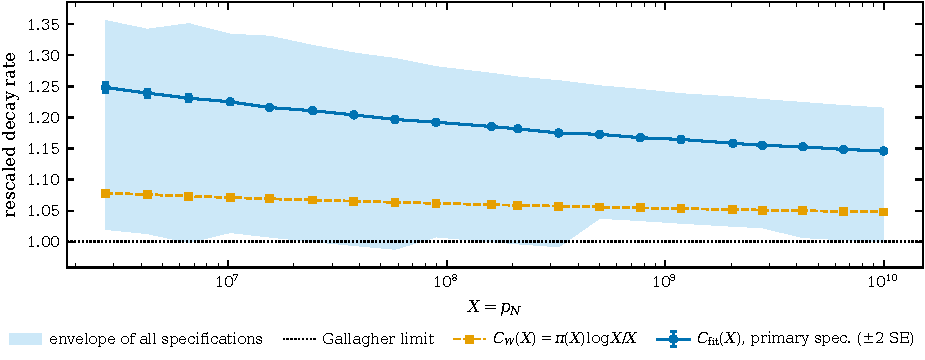
\includegraphics[width=\linewidth]{fig1_cfit}
\caption{$\Cfit(X)$ under the primary specification, the envelope generated by all \nSpecs{} specifications, and the benchmark $\CW(X)$. The envelope is wider at every scale than the change in any single specification across the whole range.}
\label{fig:cfit}
\end{figure}

\subsection{The specification grid}
\label{sec:grid}

We recomputed $\Cfit(X)$ at all scales under \nSpecs{} specifications: three estimators (the Poisson model; weighted least squares on $\log(f/H)$ with weights $|L(g;N)|$; unweighted least squares), two lower cutoffs ($g\ge2$, $g\ge4$) and six upper cutoffs ($g\le c\logX$, $c=1,\dots,6$). Each is defensible and versions of each appear in the computational literature \cite{Brent1974,Wolf2011,Wolf2014}. The window runs to $c=6$ because Wolf's published fit, described as taken over the linear portions of a semi-logarithmic plot, turns out to correspond to $c$ near $6$; a grid stopping at $c=4$ would not cover the literature it is meant to bracket. Table~\ref{tab:specgrid} and Figure~\ref{fig:specgrid} summarise the grid.

\begin{table}[tbp]
\centering\footnotesize
\caption{Sensitivity of $\Cfit$ to window and estimator. ``mon.'' records whether $\Cfit$ decreases (dec.) or increases (inc.) at every one of the \nScales{} scales, and ``first'' and ``last'' are its values at the smallest and largest scale. The full grid is in the released file \texttt{specification\_grid.csv}.}
\label{tab:specgrid}
\begin{tabular}{@{}cl rrr c@{\qquad} cl rrr c@{}}
\toprule
\multicolumn{6}{c}{$g \geq 2$} & \multicolumn{6}{c}{$g \geq 4$} \\
\cmidrule(r){1-6}\cmidrule(l){7-12}
window & est. & first & last & net & mon. & window & est. & first & last & net & mon. \\
\midrule
$1\log X$ & OLS & 1.0269 & 1.0036 & -0.0233 & -- & $1\log X$ & OLS & 1.1342 & 1.0486 & -0.0856 & -- \\
$1\log X$ & Poisson & 1.0197 & 1.0001 & -0.0196 & -- & $1\log X$ & Poisson & 1.1333 & 1.0476 & -0.0857 & -- \\
$1\log X$ & WLS & 1.0213 & 0.9999 & -0.0214 & -- & $1\log X$ & WLS & 1.1326 & 1.0462 & -0.0864 & -- \\
$2\log X$ & OLS & 1.1630 & 1.1277 & -0.0352 & -- & $2\log X$ & OLS & 1.1972 & 1.1443 & -0.0529 & -- \\
$2\log X$ & Poisson & 1.1404 & 1.1031 & -0.0373 & -- & $2\log X$ & Poisson & 1.1877 & 1.1237 & -0.0640 & -- \\
$2\log X$ & WLS & 1.1402 & 1.1030 & -0.0372 & -- & $2\log X$ & WLS & 1.1858 & 1.1231 & -0.0627 & -- \\
$3\log X$ & OLS & 1.2728 & 1.1616 & -0.1112 & -- & $3\log X$ & OLS & 1.2937 & 1.1706 & -0.1231 & -- \\
$3\log X$ & Poisson & 1.2138 & 1.1314 & -0.0824 & dec. & $3\log X$ & Poisson & 1.2483 & 1.1460 & -0.1023 & dec. \\
$3\log X$ & WLS & 1.2122 & 1.1313 & -0.0809 & dec. & $3\log X$ & WLS & 1.2458 & 1.1456 & -0.1002 & dec. \\
$4\log X$ & OLS & 1.3041 & 1.1888 & -0.1152 & dec. & $4\log X$ & OLS & 1.3174 & 1.1947 & -0.1227 & dec. \\
$4\log X$ & Poisson & 1.2356 & 1.1472 & -0.0884 & dec. & $4\log X$ & Poisson & 1.2664 & 1.1596 & -0.1068 & dec. \\
$4\log X$ & WLS & 1.2331 & 1.1469 & -0.0862 & dec. & $4\log X$ & WLS & 1.2633 & 1.1590 & -0.1043 & dec. \\
$5\log X$ & OLS & 1.3449 & 1.2013 & -0.1437 & dec. & $5\log X$ & OLS & 1.3549 & 1.2054 & -0.1495 & dec. \\
$5\log X$ & Poisson & 1.2490 & 1.1538 & -0.0952 & dec. & $5\log X$ & Poisson & 1.2778 & 1.1652 & -0.1126 & dec. \\
$5\log X$ & WLS & 1.2453 & 1.1533 & -0.0921 & dec. & $5\log X$ & WLS & 1.2741 & 1.1646 & -0.1095 & dec. \\
$6\log X$ & OLS & 1.3486 & 1.2119 & -0.1367 & -- & $6\log X$ & OLS & 1.3558 & 1.2150 & -0.1408 & -- \\
$6\log X$ & Poisson & 1.2517 & 1.1572 & -0.0945 & dec. & $6\log X$ & Poisson & 1.2797 & 1.1682 & -0.1115 & dec. \\
$6\log X$ & WLS & 1.2479 & 1.1565 & -0.0915 & dec. & $6\log X$ & WLS & 1.2759 & 1.1674 & -0.1085 & dec. \\
\bottomrule
\end{tabular}
\end{table}

\begin{figure}[tbp]
\centering
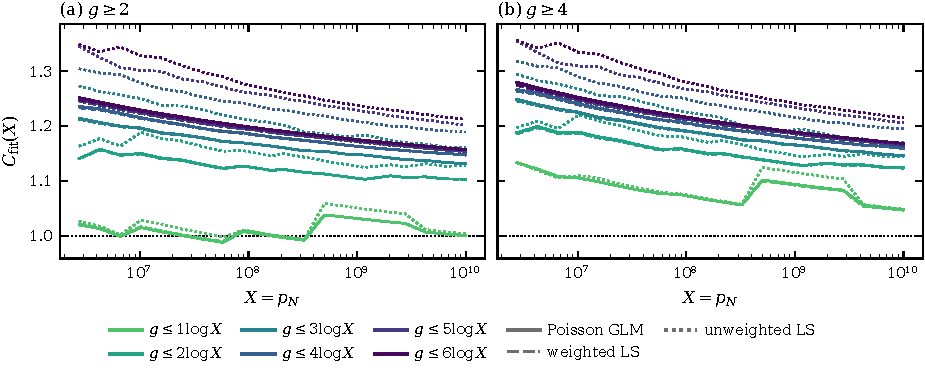
\includegraphics[width=\linewidth]{fig2_specgrid}
\caption{All \nSpecs{} specifications across the \nScales{} scales: colour is the window, line style the estimator. The vertical spread at fixed $X$ exceeds the change of any one curve across the range.}
\label{fig:specgrid}
\end{figure}

Four things follow. First, the spread of $\Cfit$ across specifications at a single $X$ lies between $\spreadMin$ and $\spreadMax$, whereas the total change under the primary specification over four decades is $\netChangePrimary$: the analyst's choice moves the statistic further than the computation does. Second, monotonicity is a property of the specification, not of the data: all \nSpecs{} decrease on net, but only \nMonoDec{} decrease at every one of the \nScales{} scales, so whether one reports a clean monotone approach depends on the window. Third, the value at $X=10^{10}$ ranges from $\narrowLast$ under the narrowest window to $\envMaxLast$ under the widest, spanning the Gallagher value itself: the adjusted frequency is flatter than exponential at small $g$ and steeper in the tail, so the ``decay rate'' is largely a choice of which part of a non-exponential curve to call the exponent. Fourth, and most directly, the published value is recovered from our own data by a change of specification. Wolf \cite{Wolf2011} reports $s$ falling from $\wolfPublished$ to $1.136$ as $X$ runs from $2^{28}$ to $2^{48}$. At our scale nearest the start of that range, $X=\wolfX$, the primary specification gives $s=\wolfOurs$ while the grid spans $[\wolfEnvMin,\wolfEnvMax]$, so the published value falls \wolfInside{} it; the closest specification, $g\ge\wolfBestGmin$ with $g\le\wolfBestC\logX$ fitted by \wolfBestEst{}, gives $\wolfBestS$, which agrees with the published $\wolfPublished$ to four decimal places. That combination is what Wolf's own description of the procedure implies. The published number is therefore accounted for by the specification alone: it need not indicate a constant, and our lower values under a different specification need not refute one.

We conclude that the question ``does $\Cfit(X)$ converge to $1$?'' is not well posed, and that no extension of the computational range will make it so. This answers Q1.

\section{Window-free local diagnostics}
\label{sec:local}

\subsection{Differencing the census}

Two problems afflict Section~\ref{sec:cfit}: the window, and the fact that every cumulative statistic over $[2,X]$ is a mixture over scales, since $\log t$ varies by a factor above twenty across that interval. Because the census stores cumulative layer occupancies at \nScales{} checkpoints, the difference of consecutive snapshots is the exact gap distribution on $I_k=(X_{k-1},X_k]$. Consecutive checkpoints are a factor of about $1.5$ apart, so $\log t$ varies by under two per cent within $I_k$. The nineteen differenced distributions are local, and they are supported on disjoint sets of primes. The primes are deterministic, so ``independence'' here means independence under the multinomial resampling model of Section~\ref{sec:uncertainty}; that is the sense in which the significance statements below are made.

On each $I_k$ we compute, with no window and no estimator, the mean gap $m_1$, the moment ratios
\begin{equation}
\Etwo=\frac{m_2}{2m_1^2},\qquad \Ethree=\frac{m_3}{6m_1^3},
\end{equation}
which equal $1$ for an exponential law (Appendix~\ref{app:lean}), and the Kolmogorov discrepancy
\begin{equation}
D=\sup_g\bigl|S(g)-e^{-g/m_1}\bigr|
\end{equation}
between the empirical survival function and the exponential with the same mean. $D$ is a discrepancy, not a test statistic: the comparison law is fitted from the same data, so the Kolmogorov null distribution does not apply, and we attach a bootstrap standard error instead. Gaps take values in $2\mathbb{Z}$, so $e^{-g/m_1}$ evaluates the continuous law at the left endpoint of the cell $(g,g+2]$; we also report the midpoint convention $e^{-(g+1)/m_1}$. Because $S(g)$ sums over gaps, the oscillation $H(g)$ is averaged out and no singular-series correction is needed here.

The effective scale of $I_k$ is $\log\Xeff=\bigl(X_k(\log X_k-1)-X_{k-1}(\log X_{k-1}-1)\bigr)/(X_k-X_{k-1})$, the mean of $\log t$ over the interval. (The density-weighted mean $(X_k-X_{k-1})/(\li X_k-\li X_{k-1})$ differs from it by under $0.002$ on every interval.)

\subsection{Results}

Table~\ref{tab:local} gives the local diagnostics and Figure~\ref{fig:local} plots them. The first observation is a validation: the local mean gap agrees with $\log\Xeff$ to within $5\times10^{-4}$ in relative terms on every interval (ratio in $[\ratioMin,\ratioMax]$). This is the Prime Number Theorem reproduced locally, and a sharper check on the census than matching tabulated $\pi(X)$ values \cite{DelegliseRivat1996}, because it tests the gap bookkeeping at every scale.

\begin{table}[tbp]
\centering\small
\caption{Window-free local diagnostics on the nineteen differenced intervals. $\Etwo$, $\Ethree$ equal $1$ and $D$ equals $0$ for an exponential law; $D$ uses the left-endpoint convention. The column $\log\Xeff/m_1$ is a local test of the Prime Number Theorem.}
\label{tab:local}
\begin{tabular}{rrr c c c c c c}
\toprule
$k$ & $X_{k-1}$ & $X_k$ & gaps & $m_1$ & $\log X_{\mathrm{eff}}/m_1$ & $E_2$ & $E_3$ & $D$ \\
\midrule
1 & 2\,750\,159 & 4\,262\,509 & 100\,411 & 15.0616 & 1.00004 & 0.84606 & 0.68323 & 0.05643 \\
2 & 4\,262\,509 & 6\,601\,211 & 150\,823 & 15.5063 & 0.99959 & 0.84574 & 0.68190 & 0.05767 \\
3 & 6\,601\,211 & 10\,213\,061 & 226\,544 & 15.9434 & 0.99959 & 0.85066 & 0.69260 & 0.05581 \\
4 & 10\,213\,061 & 15\,485\,863 & 322\,222 & 16.3638 & 0.99987 & 0.85195 & 0.69415 & 0.05521 \\
5 & 15\,485\,863 & 24\,373\,961 & 529\,183 & 16.7959 & 1.00020 & 0.85602 & 0.70253 & 0.05483 \\
6 & 24\,373\,961 & 37\,614\,323 & 767\,734 & 17.2460 & 0.99974 & 0.85804 & 0.70583 & 0.05417 \\
7 & 37\,614\,323 & 57\,995\,527 & 1\,153\,178 & 17.6739 & 1.00006 & 0.86189 & 0.71499 & 0.05339 \\
8 & 57\,995\,527 & 89\,359\,883 & 1\,732\,138 & 18.1073 & 1.00001 & 0.86536 & 0.72097 & 0.05227 \\
9 & 89\,359\,883 & 160\,481\,183 & 3\,817\,767 & 18.6290 & 1.00002 & 0.86792 & 0.72633 & 0.05148 \\
10 & 160\,481\,183 & 211\,733\,111 & 2\,691\,997 & 19.0386 & 1.00000 & 0.87070 & 0.73230 & 0.05084 \\
11 & 211\,733\,111 & 325\,619\,971 & 5\,870\,027 & 19.4014 & 1.00000 & 0.87232 & 0.73538 & 0.05020 \\
12 & 325\,619\,971 & 500\,465\,113 & 8\,817\,104 & 19.8302 & 1.00006 & 0.87457 & 0.73991 & 0.04952 \\
13 & 500\,465\,113 & 768\,813\,691 & 13\,243\,776 & 20.2622 & 0.99994 & 0.87689 & 0.74453 & 0.04882 \\
14 & 768\,813\,691 & 1\,180\,371\,793 & 19\,892\,881 & 20.6887 & 1.00006 & 0.87864 & 0.74798 & 0.04822 \\
15 & 1\,180\,371\,793 & 2\,038\,074\,743 & 40\,484\,215 & 21.1861 & 1.00004 & 0.88105 & 0.75266 & 0.04743 \\
16 & 2\,038\,074\,743 & 2\,778\,410\,251 & 34\,277\,704 & 21.5982 & 1.00000 & 0.88292 & 0.75633 & 0.04676 \\
17 & 2\,778\,410\,251 & 4\,259\,763\,509 & 67\,414\,809 & 21.9737 & 1.00001 & 0.88478 & 0.76026 & 0.04621 \\
18 & 4\,259\,763\,509 & 6\,528\,037\,501 & 101\,260\,758 & 22.4003 & 1.00003 & 0.88638 & 0.76339 & 0.04566 \\
19 & 6\,528\,037\,501 & 9\,999\,999\,967 & 152\,099\,240 & 22.8270 & 1.00003 & 0.88815 & 0.76691 & 0.04505 \\
\bottomrule
\end{tabular}
\end{table}

\begin{figure}[tbp]
\centering
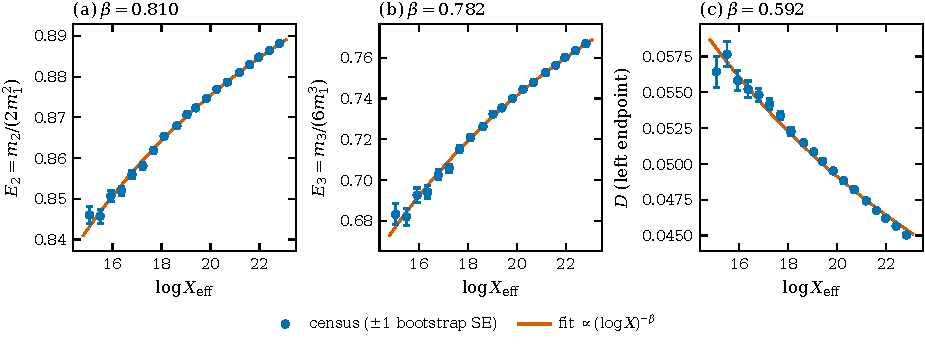
\includegraphics[width=\linewidth]{fig3_local}
\caption{The local diagnostics against $\log\Xeff$ with bootstrap standard errors (mostly smaller than the markers) and the fitted power laws $|{\rm stat}-{\rm limit}|\propto(\logX)^{-\beta}$.}
\label{fig:local}
\end{figure}

The substantive result is that $\Etwo$ rises from $\EtwoFirst$ to $\EtwoLast$, $\Ethree$ from $\EthreeFirst$ to $\EthreeLast$, and $D$ falls from $\DFirst$ to $\DLast$. Prime gaps at these scales are under-dispersed relative to the exponential law ($\Etwo<1$: more regular than a Poisson process), and the under-dispersion is shrinking. This is the finite-$X$ counterpart of Cohen's asymptotic statement \cite{Cohen2025}: the moments approach their exponential values while the distribution remains non-exponential throughout the range.

Under the midpoint convention $D$ falls from $\DmidFirst$ to $\DmidLast$, roughly double in absolute terms with the same monotone decrease; the absolute level of $D$ is convention-dependent and only its trend should be read. A Cram\'er--von Mises distance $W^2$, which weights the whole distribution rather than its point of maximal deviation, decreases at all \nSteps{} steps (Table~\ref{tab:steps}).

On the rate of approach, the deviations are not well described by $c/\logX$. A log-log regression of each deviation on $\log\Xeff$ gives exponents $\betaEtwo\pm\betaEtwoSE$ for $1-\Etwo$, $\betaEthree\pm\betaEthreeSE$ for $1-\Ethree$ and $\betaD\pm\betaDSE$ for $D$: fractional powers of $\logX$. The exponent for $D$ depends on the continuity convention (the midpoint form gives $0.67\pm0.01$), which is one more reason to prefer the moment ratios. Extrapolated, $1-\Etwo$ would still be about $\EtwoAtFifty$ at $\logX=50$ and $\EtwoAtTwoHundred$ at $\logX=200$. We are extrapolating from under one decade in $\logX$ and do not offer these as predictions; they quantify how far out of reach a decisive computation is.

\subsection{Uncertainty and significance}
\label{sec:uncertainty}

We attach a nonparametric bootstrap standard error to each statistic by resampling the layer counts on each interval from the multinomial distribution they define ($2000$ resamples per interval) \cite{EfronTibshirani1993}. Because the intervals are disjoint, the standard error of a consecutive difference is the root sum of squares of the two. Table~\ref{tab:uncertainty} gives six representative intervals and Table~\ref{tab:steps} the step tests.

\begin{table}[tbp]
\centering\small
\caption{Bootstrap standard errors at six representative intervals; all nineteen are in \texttt{local\_diagnostics.csv}.}
\label{tab:uncertainty}
\begin{tabular}{r c c c c c}
\toprule
$k$ & $\log X_{\mathrm{eff}}$ & $E_2$ (SE) & $E_3$ (SE) & $D_{\mathrm{left}}$ (SE) & $D_{\mathrm{mid}}$ (SE) \\
\midrule
1 & 15.062 & 0.84606 (0.00201) & 0.68323 (0.00508) & 0.05643 (0.00109) & 0.10569 (0.00109) \\
5 & 16.799 & 0.85602 (0.00092) & 0.70253 (0.00242) & 0.05483 (0.00045) & 0.10038 (0.00045) \\
9 & 18.629 & 0.86792 (0.00037) & 0.72633 (0.00098) & 0.05148 (0.00017) & 0.09365 (0.00017) \\
13 & 20.261 & 0.87689 (0.00020) & 0.74453 (0.00055) & 0.04882 (0.00009) & 0.08835 (0.00009) \\
16 & 21.598 & 0.88292 (0.00013) & 0.75633 (0.00035) & 0.04676 (0.00005) & 0.08436 (0.00005) \\
19 & 22.828 & 0.88815 (0.00006) & 0.76691 (0.00017) & 0.04505 (0.00002) & 0.08102 (0.00002) \\
\bottomrule
\end{tabular}
\end{table}

\begin{table}[tbp]
\centering\small
\caption{Consecutive-step and end-to-end tests. A step counts as ``toward the limit'' when the statistic moves toward its exponential value; $z$ is the change divided by the root-sum-square of the two bootstrap standard errors. $\beta$ is the fitted exponent in $(\logX)^{-\beta}$.}
\label{tab:steps}
\begin{tabular}{l c c c c c c}
\toprule
statistic & steps toward limit & median $z$ & min $z$ & end-to-end change & end-to-end $z$ & exponent $\beta$ \\
\midrule
$E_2$ & 17/18 & 4.5 & -0.12 & +0.0421 $\pm$ 0.0020 & 21 & 0.810 $\pm$ 0.011 \\
$E_3$ & 17/18 & 3.7 & -0.20 & +0.0837 $\pm$ 0.0051 & 16 & 0.782 $\pm$ 0.012 \\
$D_{\mathrm{left}}$ & 17/18 & 2.8 & -0.89 & -0.0114 $\pm$ 0.0011 & 10 & 0.592 $\pm$ 0.017 \\
$D_{\mathrm{mid}}$ & 17/18 & 5.5 & -0.17 & -0.0247 $\pm$ 0.0011 & 23 & 0.666 $\pm$ 0.010 \\
$W^2$ & 18/18 & 6.1 & 0.47 & -0.0012 $\pm$ 0.0000 & 25 & -- \\
\bottomrule
\end{tabular}
\end{table}

Three statements can be made. Of the \nSteps{} consecutive steps, \towardEtwo{} move each of $\Etwo$, $\Ethree$ and $D$ toward the Gallagher prediction. The single exception is the first step, from $I_1$ to $I_2$, where $\Etwo$ falls ($z=\zFirstStepEtwo$), $\Ethree$ falls ($z=\zFirstStepEthree$) and $D$ rises ($z=\zFirstStepD$): all within one standard error of no change, at the smallest and noisiest scales in the census. Where the steps do move in the predicted direction they mostly do so significantly: the median $z$ is $\medzEtwo$ for $\Etwo$, $\medzEthree$ for $\Ethree$ and $\medzD$ for $D$. The end-to-end change is large relative to its own uncertainty: $z\approx\zEtwoEnd$ for $\Etwo$, $\zEthreeEnd$ for $\Ethree$ and $\zDEnd$ for $D$.

What we claim is therefore this. Three statistics that involve no analyst choice move toward the Gallagher prediction across four decades, by margins of ten to twenty standard errors end to end, with a single within-noise exception at the smallest scale. That is evidence for convergence of a kind the fitted rate cannot supply. It is not proof, and it does not exclude a limit differing slightly from the exponential one. This answers Q2.

\section{Spatial localisation: a derived crossover}
\label{sec:spatial}

\subsection{The relative spatial mean}

Define the layer mean $\mu(g;N)=|L(g;N)|^{-1}\sum_{p\in L(g;N)}p$, the overall mean $\mu(N)=(N-1)^{-1}(p_2+\cdots+p_N)$, and
\begin{equation}
R(g;N)=\frac{\mu(g;N)}{\mu(N)}.
\end{equation}
$R$ measures whether the primes carrying gap $g$ sit on average earlier ($R<1$) or later ($R>1$) in the sequence than a typical prime up to the $N$th. It is a direct empirical mean, with no fitting, no window and no arithmetic correction, and since the layer prime-sums are exact integers it is reproducible to full precision. The crossover $g^*(X)$ is the gap at which $R=1$.

The census also stores the layer sums of squares, which is what makes a standard error possible. Since $\mu(N)$ contains $\mu(g;N)$, the two are correlated; writing $w=|L(g;N)|/(N-1)$ and splitting the primes into layer $g$ and the rest, the delta method gives
\begin{equation}
\operatorname{Var}(R)=(1-w)^2\Bigl[\frac{\mu_r^2\sigma_g^2}{n_g}+\frac{\mu_g^2\sigma_r^2}{n_r}\Bigr]\Big/\mu(N)^4,
\label{eq:varR}
\end{equation}
every ingredient of which is an exact integer moment. As with Section~\ref{sec:local}, these are standard errors of a sampling model in which layer membership is random: the primes are deterministic, so \eqref{eq:varR} quantifies the arithmetic fluctuation of a layer rather than a probability about the primes. The released self-test checks \eqref{eq:varR} against a direct bootstrap over the actual primes of a layer at a scale small enough to enumerate them.

\subsection{A parameter-free density model}

Take the density of primes near $t$ to be $1/\log t$ and, following \eqref{eq:wolf} with $\pi(t)/t$ replaced by $1/\log t$, the conditional probability that a prime near $t$ carries outgoing gap $g$ to be $(C_2H(g)/\log t)\exp(-g/\log t)$. The layer-$g$ density is the product, and $C_2H(g)$ cancels identically in a ratio of means. Writing $w_g(t)=\exp(-g/\log t)/(\log t)^2$,
\begin{equation}
R_{\rm model}(g;X)=\frac{\int_2^X t\,w_g(t)\,dt\big/\int_2^X w_g(t)\,dt}{\int_2^X t/\log t\,dt\big/\int_2^X dt/\log t}.
\label{eq:model}
\end{equation}
The model has nothing to tune, so agreement with the data is a test rather than a fit. Substituting $t=e^{L-v}$, $L=\logX$, expanding to first order in $1/L$ and writing $a=g/L^2$ gives (Appendix~\ref{app:expansion})
\begin{equation}
R_{\rm model}=1+\frac{a}{2}-\frac{1}{2L}+O(L^{-2}).
\label{eq:firstorder}
\end{equation}
Setting $R=1$ gives $a=1/L$, that is $g^*=\logX+o(\logX)$: the crossover sits at the mean gap. In $x=g/\logX$ the correction takes the scaling form
\begin{equation}
R(g;N)=1+\frac{\Phi(x)}{\logX}+o\Bigl(\frac1{\logX}\Bigr),\qquad \Phi(1)=0,
\label{eq:scaling}
\end{equation}
with $\Phi(x)=(x-1)/2$ to first order. Both the abscissa and the amplitude must be rescaled, the latter by $\logX$.

The replacement of $\pi(t)/t$ by $1/\log t$ is a simplification. The two differ by the factor $\CW(t)\approx1.05$ at these scales, which is of the same order as the $O(1)$ corrections discussed below, so we evaluate \eqref{eq:model} numerically for both envelopes (the released \texttt{spatial.py} uses a quadrature stable at arbitrarily large $L$).

\subsection{The crossover}
\label{sec:crossover}

Because $R(g)$ is nearly flat near the crossing and single layers carry arithmetic fluctuations, $g^*$ is located by a linear regression of $R$ on $g$ and solved for $R=1$. The regression window is an analyst choice. The primary locator uses the scale-invariant window $0.6\le g/\logX\le1.4$, which is the same window in scaling units at every scale and matches the linear form of $\Phi$ to first order; we also report the windows $[0.7,1.3]$ and $[0.5,1.5]$, the bands $|R-1|<b$ for $b\in\{0.02,0.03,0.05\}$ used in an earlier version of this work, and plain interpolation between the two even gaps bracketing $R=1$. Table~\ref{tab:crossover} and Figure~\ref{fig:crossover} give the results.

\begin{table}[tbp]
\centering\footnotesize
\caption{The computed crossover under six locators. The last two columns use the primary locator (window $x\in[0.6,1.4]$, bold).}
\label{tab:crossover}
\begin{tabular}{rr ccc ccc c c}
\toprule
$X=p_N$ & $\log X$ & \multicolumn{3}{c}{window in $x$} & \multicolumn{3}{c}{band in $R$} & \multicolumn{2}{c}{weighted fit} \\
\cmidrule(lr){3-5}\cmidrule(lr){6-8}
 & & $[0.7,1.3]$ & $[0.6,1.4]$ & $[0.5,1.5]$ & 0.02 & 0.03 & 0.05 & $g^*$ (WLS) & $\log X-g^*$ \\
\midrule
2\,750\,159 & 14.827 & 13.79 & \textbf{14.26} & 14.57 & 13.54 & 14.57 & 14.18 & 14.13 $\pm$ 0.45 & 0.69 \\
4\,262\,509 & 15.265 & 14.29 & \textbf{14.54} & 15.03 & 14.29 & 14.82 & 14.51 & 14.55 $\pm$ 0.39 & 0.71 \\
6\,601\,211 & 15.703 & 14.52 & \textbf{14.98} & 15.48 & 14.49 & 15.48 & 15.15 & 14.94 $\pm$ 0.38 & 0.76 \\
10\,213\,061 & 16.139 & 15.05 & \textbf{15.44} & 15.37 & 15.52 & 15.48 & 15.25 & 15.49 $\pm$ 0.43 & 0.65 \\
15\,485\,863 & 16.555 & 15.49 & \textbf{16.00} & 15.96 & 15.72 & 15.84 & 15.63 & 15.89 $\pm$ 0.43 & 0.66 \\
24\,373\,961 & 17.009 & 16.11 & \textbf{16.11} & 16.28 & 16.11 & 16.18 & 16.07 & 16.11 $\pm$ 0.58 & 0.89 \\
37\,614\,323 & 17.443 & 16.65 & \textbf{16.44} & 16.56 & 16.48 & 16.62 & 16.49 & 16.38 $\pm$ 0.34 & 1.06 \\
57\,995\,527 & 17.876 & 16.97 & \textbf{16.88} & 17.10 & 16.91 & 17.03 & 16.79 & 16.87 $\pm$ 0.30 & 1.01 \\
89\,359\,883 & 18.308 & 17.84 & \textbf{17.66} & 17.69 & 17.66 & 17.62 & 17.31 & 17.66 $\pm$ 0.39 & 0.65 \\
160\,481\,183 & 18.894 & 18.20 & \textbf{18.12} & 18.31 & 18.12 & 18.16 & 17.84 & 18.12 $\pm$ 0.21 & 0.77 \\
211\,733\,111 & 19.171 & 18.51 & \textbf{18.38} & 18.56 & 18.44 & 18.42 & 18.09 & 18.36 $\pm$ 0.25 & 0.81 \\
325\,619\,971 & 19.601 & 19.01 & \textbf{18.94} & 19.11 & 19.01 & 18.93 & 18.54 & 18.95 $\pm$ 0.29 & 0.65 \\
500\,465\,113 & 20.031 & 19.28 & \textbf{19.53} & 19.43 & 19.54 & 19.23 & 18.98 & 19.55 $\pm$ 0.38 & 0.48 \\
768\,813\,691 & 20.460 & 19.81 & \textbf{19.96} & 19.84 & 19.93 & 19.52 & 19.38 & 19.97 $\pm$ 0.33 & 0.49 \\
1\,180\,371\,793 & 20.889 & 20.15 & \textbf{20.29} & 20.19 & 20.23 & 19.91 & 19.77 & 20.30 $\pm$ 0.32 & 0.58 \\
2\,038\,074\,743 & 21.435 & 20.74 & \textbf{20.82} & 20.68 & 20.82 & 20.51 & 20.32 & 20.81 $\pm$ 0.28 & 0.62 \\
2\,778\,410\,251 & 21.745 & 21.20 & \textbf{21.16} & 21.02 & 21.18 & 20.78 & 20.65 & 21.14 $\pm$ 0.28 & 0.61 \\
4\,259\,763\,509 & 22.172 & 21.76 & \textbf{21.69} & 21.48 & 21.54 & 21.23 & 21.09 & 21.65 $\pm$ 0.27 & 0.52 \\
6\,528\,037\,501 & 22.599 & 22.17 & \textbf{22.04} & 21.86 & 21.88 & 21.68 & 21.52 & 22.00 $\pm$ 0.27 & 0.60 \\
9\,999\,999\,967 & 23.026 & 22.56 & \textbf{22.34} & 22.31 & 22.28 & 22.09 & 21.94 & 22.37 $\pm$ 0.27 & 0.66 \\
\bottomrule
\end{tabular}
\end{table}

\begin{figure}[tbp]
\centering
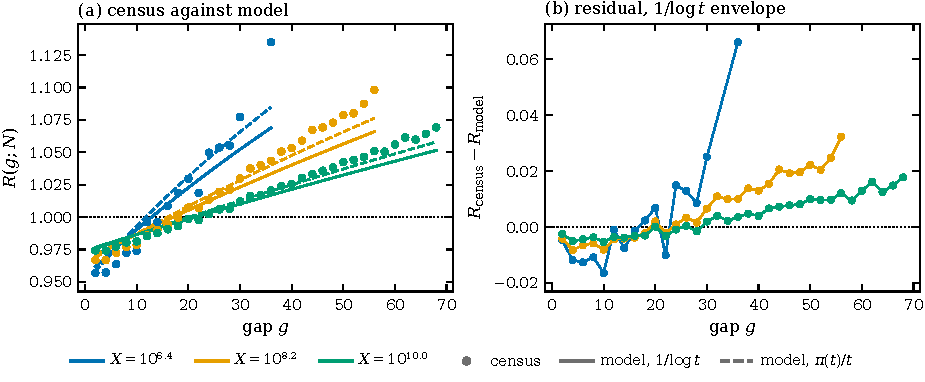
\includegraphics[width=\linewidth]{fig4_model}
\caption{(a) $R(g;N)$ at three scales against the parameter-free model with the $1/\log t$ envelope (solid) and the $\pi(t)/t$ envelope (dashed). (b) Residual from the $1/\log t$ model; it shrinks with $X$ in absolute terms because the whole effect scales as $1/\logX$ (see Figure~\ref{fig:collapse}(c) for the relative comparison).}
\label{fig:model}
\end{figure}

\begin{figure}[tbp]
\centering
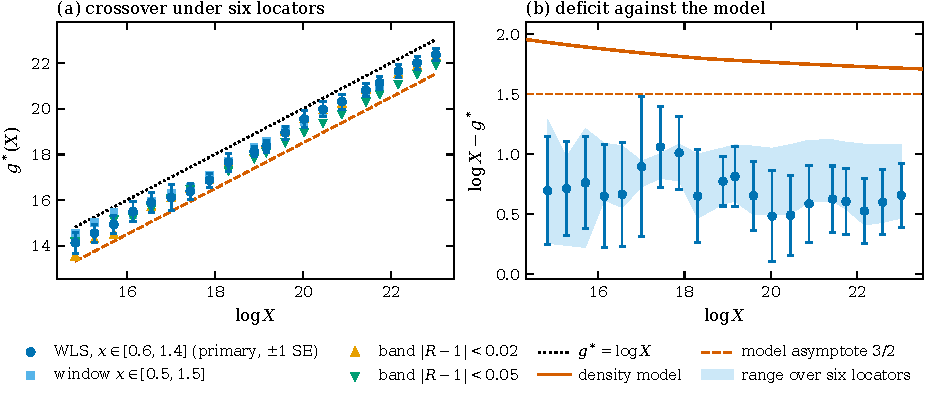
\includegraphics[width=\linewidth]{fig6_crossover}
\caption{(a) The crossover $g^*(X)$ under four of the six locators, with $g^*=\logX$ and the model's asymptote $g^*=\logX-3/2$. (b) The deficit $\logX-g^*$: census (primary locator, with the range over all six locators shaded) against the numerical model. The model's $O(1)$ constant is not reproduced.}
\label{fig:crossover}
\end{figure}

The primary locator is now a weighted least-squares fit using the standard errors \eqref{eq:varR}, which also yields a standard error for $g^*$ by the delta method; the unweighted locators are retained for comparison. Two conclusions are robust to the locator. The crossover rises with $X$ (from $\gstarFirst$ to $\gstarLast$) and tracks $\logX$: $g^*/\logX$ lies between $\ratioAllMin$ and $\ratioAllMax$ over all scales and all six locators. The deficit $\logX-g^*$ is $O(1)$, lying between $\deficitMin$ and $\deficitMax$.

The error bars change what can be claimed, in both directions. At the largest scale, $g^*=\gstarLast\pm\gstarLastSE$ against $\logX=23.026$, so $g^*/\logX=\ratioLastVal\pm\ratioLastSE$ and the naive reading $g^*=\logX$ is excluded at $\sigmaUnity$ standard errors: the crossover sits slightly but detectably below the mean gap. In the other direction, we withdraw any claim about a trend in the deficit. An earlier version of this work reported an upward drift, which is what the band $b=0.03$ produces; the band $b=0.02$ produces a downward drift and the scale-invariant windows produce none. More fundamentally, the \nScales{} scales are nested, since the census at $X_k$ contains every prime used at $X_{k-1}$, so the $g^*$ series is strongly autocorrelated and a trend test that treats the scales as independent is invalid. Unlike the frequency statistics of Section~\ref{sec:local}, the spatial statistic cannot be localised to fix this: $R$ acquires its dynamic range from the variation of $\log t$ across the whole interval $[2,X]$, and on one differenced interval $R$ varies by under $0.005$ against $0.38$ cumulatively. Nesting is intrinsic to the statistic, and we make only single-scale statements about it.

Evaluating the model \eqref{eq:model} numerically gives a deficit of $\modelDeficitTen$ at $\logX=23$, decreasing to $\modelDeficitHundred$ at $\logX=230$ and to $1.5004$ at $\logX=10^{4}$, so $g^*=\logX-3/2+o(1)$ for the model. The census gives $\deficitLastVal\pm\deficitLastSE$ at the largest scale, which excludes $3/2$ at $\sigmaModel$ standard errors. The model therefore predicts the leading term correctly and the $O(1)$ term incorrectly, and this is now a measurement rather than an impression; the $\pi(t)/t$ envelope does worse still (deficit $2.78$ at $\logX=23$).

\subsection{The scaling collapse}

Figure~\ref{fig:collapse} tests \eqref{eq:scaling}. Panel (a) shows $R$ against $g$: the curves are distinct and the crossing moves rightward with $X$. Panel (b) rescales the abscissa alone: the crossings collapse onto $x\approx0.96$, but the profiles do not, since the amplitude of $R-1$ shrinks with $X$. Panel (c) plots $\logX\,(R-1)$ against $x$, the full rescaling the model requires: the \nScales{} curves collapse onto a single increasing profile with $\Phi(1)\approx0$. The residual spread in panel (c) is a downward drift of the slope from about $0.91$ to $0.78$ across four decades (fitted over $0.3\le x\le1.5$), consistent with the $O(1/\log^2X)$ terms neglected in the derivation. We regard the collapse as established for $x\lesssim2$ and suggestive beyond it.

\begin{figure}[tbp]
\centering
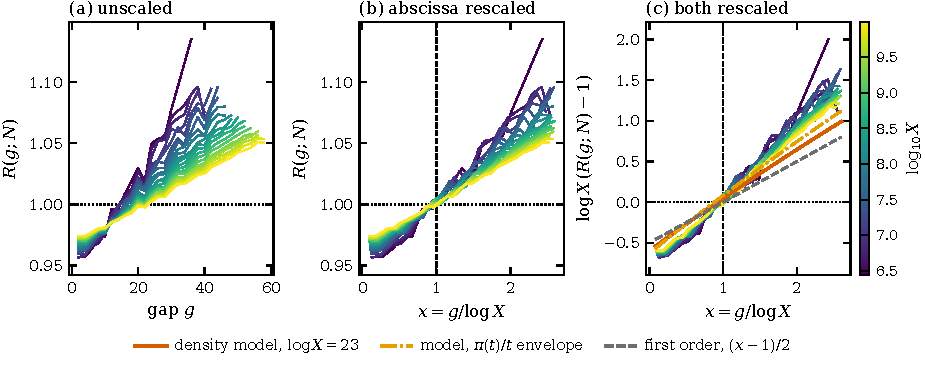
\includegraphics[width=\linewidth]{fig5_collapse}
\caption{The scaling collapse. (a) $R$ against $g$ at all \nScales{} scales; (b) abscissa rescaled by $\logX$; (c) abscissa and amplitude rescaled. Panel (c) also shows the full numerical model at $\logX=23$ for both envelopes and the first-order profile $(x-1)/2$: the model reproduces the crossing and the shape, not the slope.}
\label{fig:collapse}
\end{figure}

Panel (c) also exposes the model's limitation. In the collapsed variable the model profile at $\logX=23$ has slope $\ampSlopeModel$ (tending to the first-order value $1/2$ as $L\to\infty$) whereas the census profile has slope $\ampSlopeData$ at the same scale. Fitting both over the same window $0.3\le x\le1.5$ at every scale, the ratio of census slope to model slope is $\ampRatio\pm\ampRatioSD$ (mean and standard deviation over the \nScales{} scales, range $[\ampRatioMin,\ampRatioMax]$), with a total drift across the range smaller than that standard deviation. For the $\pi(t)/t$ envelope the ratio is $\ampRatioPi\pm\ampRatioPiSD$. Quoting residuals in $R$, as Figure~\ref{fig:model}(b) does, makes the agreement look better than it is, because $R-1$ is itself $O(1/\logX)$. The correct statement is that the model predicts the location of the crossover to about $4\%$ and the form of the scaling law, and under-predicts the amplitude by a scale-independent factor. A stable multiplicative discrepancy is what one expects if the mechanism is right and the envelope shape is wrong, and Section~\ref{sec:local} has already shown that the gap distribution at these scales is not the exponential envelope assumed in \eqref{eq:model}. Whether feeding the measured under-dispersion back into \eqref{eq:model} recovers the amplitude is an open question we have not pursued. This answers Q3.

\section{Discussion}

The two diagnostics share a mechanism: as $X$ grows the typical gap $\logX$ grows with it, and both the frequency envelope and the spatial distribution of a fixed $g$ are reshaped relative to that moving scale. What differs is how cleanly each can be measured.

On the frequency side the contribution is a caution and a replacement. The caution is that the fitted decay rate around which the plateau question has been posed \cite{Brent1974,OdlyzkoRubinsteinWolf1999,Wolf2014} is specification-dependent to a degree exceeding the effect under study. The replacement is the local diagnostics of Section~\ref{sec:local}. Our reading is that the value near $1.2$ is best understood neither as a constant nor as a slowly decaying estimate of unity, but as one summary of a distribution that is not exponential at accessible $X$, measurably under-dispersed ($\Etwo\approx\EtwoLast$ at $10^{10}$), whose departure from exponentiality decays as a fractional power of $\logX$. This is consistent with Cohen \cite{Cohen2025}, with the refinements of the Cram\'er model \cite{Cramer1936} by Granville \cite{Granville1995} and by Montgomery and Soundararajan \cite{MontgomerySoundararajan2002,MontgomerySoundararajan2004}, which predict slow and structured approach for several classical gap statistics, and with the warning of Lemke Oliver and Soundararajan \cite{LemkeOliverSoundararajan2016}. None of it bears on the bounded-gap theorems of Zhang \cite{Zhang2014} and Maynard \cite{Maynard2015}, which concern the extreme lower tail rather than the bulk studied here; for the wider background see Soundararajan \cite{Soundararajan2007}.

On the spatial side the crossover appears to be a new empirical observation and comes with a derivation. That $C_2H(g)$ cancels tells us $R(g;N)$ is insensitive to the arithmetic of $g$ and reflects only the interaction between the growth of $\log t$ and the envelope. This bounds the phenomenon's depth: the crossover is a consequence of the envelope and the prime density, not an independent arithmetic fact. Its interest is diagnostic. $R$ is measured without fitting, reproduces exactly across implementations, and its crossover location converges to its scaling form visibly faster than the frequency statistics converge to theirs. The amplitude discrepancy of Section~\ref{sec:crossover} is, we think, the most useful thing the spatial statistic has produced so far: it is a quantitative, scale-stable measurement of how far the actual gap law is from the exponential envelope, obtained without any window.

\section{Limitations}

\emph{The Gallagher limit is not established.} Section~\ref{sec:local} reports approach with end-to-end significance of ten to twenty standard errors, but at fractional-power rates: the extrapolated deviation at $\logX=50$ is still about $\EtwoAtFifty$ in $\Etwo$. Nothing here distinguishes the Gallagher limit from a limit differing from it by a few per cent.

\emph{One step is not monotone.} The transition from $I_1$ to $I_2$ moves all three statistics marginally the wrong way, within one bootstrap standard error. We report it rather than trimming the smallest interval.

\emph{The fractional exponents are descriptive.} They are least-squares fits over $\logX$ from $15$ to $23$ and we have no derivation for them. The exponent for $D$ depends on the continuity convention.

\emph{The crossover scales are nested, so only single-scale statements are made.} The deficit is measured to about $\pm\deficitLastSE$ at the largest scale, which is enough to exclude both $0$ and the model's $3/2$ but not to establish its value or any trend. The spatial statistic cannot be localised into independent samples the way the frequency statistics can (Section~\ref{sec:crossover}). The model's $3/2$ rests on numerics of a heuristic, not on an analytic second-order evaluation.

\emph{The density model under-predicts the amplitude} of $R-1$ by a factor of $\ampRatio\pm\ampRatioSD$, with no trend across scales. It assumes the exponential envelope exactly and uses $1/\log t$ for the prime density; it should also fail in the far tail $g\gtrsim1.5\logX$, where layers are sparse and the maximal-gap heuristics of Kourbatov and Wolf \cite{KourbatovWolf2019} take over, and Figure~\ref{fig:model} shows that it does.

\emph{Independence is model-based.} The primes are deterministic. Independence of the differenced intervals holds under the multinomial resampling model, and the $z$-scores of Section~\ref{sec:local} should be read in that sense. The same caveat applies to \eqref{eq:varR} and to the standard errors reported for $\Cfit$, which come from the Fisher information of a Poisson model whose counts are in truth multinomial and deterministic; all of these measure arithmetic fluctuation, not sampling error in the usual sense.

\emph{The power-law exponents assume independent residuals.} They are unweighted least-squares fits on nineteen points whose residuals are visibly autocorrelated, so the quoted standard errors on $\beta$ understate the true uncertainty.

\emph{$D$ is a discrepancy, not a test statistic.} Only its trend, and the bootstrap uncertainty on that trend, should be read.

\section{Methods, verification and reproducibility}
\label{sec:methods}

\subsection{The census}

Primes were generated by a bit-packed segmented sieve of Eratosthenes over the odd integers (\texttt{fgp\_sieve.c}), of the standard form described by Crandall and Pomerance \cite{CrandallPomerance2005}. The segment window is $256$\,KiB, chosen to stay in L2 cache; base primes below $10^{5}$ are sieved once. Memory is $O(\sqrt X)$ plus one window, a few megabytes independent of $X$. Primes are streamed in increasing order, each accumulated into the layer indexed by its outgoing gap, and layer occupancies and layer prime-sums are snapshotted at \nScales{} checkpoints. The layer prime-sums are exact: their total to $10^{10}$ is about $2.2\times10^{18}$, below the unsigned 64-bit bound by a factor of eight, so the spatial means are exact rationals. The checkpoint schedule is \nScales{} geometrically spaced values of $N$ from $\Nfirst$ to $\pi(10^{10})$, with $N=10^{6}$, $9\times10^{6}$ and $10^{8}$ snapped onto the grid so that scales in the earlier literature are directly comparable. The run to $10^{10}+10^{3}$ took \sieveSeconds{} seconds on one core.

\subsection{Verification}

\emph{Prime counts and indices.} $\pi(10^{7})=664\,579$ and $\pi(10^{10})=455\,052\,511$, matching tabulated values \cite{DelegliseRivat1996,CrandallPomerance2005}; $p_{200000}=2\,750\,159$, $p_{10^{6}}=15\,485\,863$, $p_{10^{8}}=2\,038\,074\,743$; the largest prime below $10^{10}$ is $9\,999\,999\,967$.

\emph{Maximal gap.} The largest gap below $10^{10}$ is $354$, following $4\,302\,407\,359$, reproducing the first-occurrence tables of Nicely \cite{Nicely1999} and consistent with \cite{OliveiraeSilvaHerzogPardi2014}.

\emph{Local Prime Number Theorem.} On each differenced interval the mean gap agrees with $\log\Xeff$ to within $5\times10^{-4}$ relative (Table~\ref{tab:local}).

\emph{Independent reimplementation.} A second census, written from scratch in NumPy with one byte per integer, segments of $10^{8}$, and gaps taken by differencing arrays rather than by a running pointer (\texttt{verify.py}), recomputes every layer count at every checkpoint over the whole range, to $X=\verifyXmax$. All \verifyLayers{} counts agree exactly (Table~\ref{tab:verify}); the run takes \verifySeconds{} seconds. The two programs share no code, no data layout and no language, so this removes the single-implementation caveat at every one of the \nScales{} scales rather than at the smaller ones only.

The verifier had itself to be corrected before it would run to the end of the range, in a way worth recording because it is the same trap as Section~\ref{sec:census}. Sieving $[2,X]$ and then asking for the layer occupancies at $N=\pi(X)$ fails, because the layer of $p_N$ is fixed by $p_{N+1}$, which lies outside the sieved interval: at $X=10^{10}$ the next prime is $10\,000\,000\,019$. The verifier now sieves past its limit by a margin, exactly as the census does. It also aborts rather than truncating if a gap exceeds the width of the histogram.

\begin{table}[tbp]
\centering\small
\caption{Independent NumPy census against the C census: layer counts compared at each checkpoint with $X\le\verifyXmax$.}
\label{tab:verify}
\begin{tabular}{r r r r}
\toprule
checkpoint $k$ & $X$ & layers compared & mismatches \\
\midrule
0 & 2\,750\,159 & 62 & 0 \\
1 & 4\,262\,509 & 65 & 0 \\
2 & 6\,601\,211 & 70 & 0 \\
3 & 10\,213\,061 & 74 & 0 \\
4 & 15\,485\,863 & 77 & 0 \\
5 & 24\,373\,961 & 81 & 0 \\
6 & 37\,614\,323 & 85 & 0 \\
7 & 57\,995\,527 & 93 & 0 \\
8 & 89\,359\,883 & 96 & 0 \\
9 & 160\,481\,183 & 103 & 0 \\
10 & 211\,733\,111 & 108 & 0 \\
11 & 325\,619\,971 & 112 & 0 \\
12 & 500\,465\,113 & 119 & 0 \\
13 & 768\,813\,691 & 127 & 0 \\
14 & 1\,180\,371\,793 & 129 & 0 \\
15 & 2\,038\,074\,743 & 143 & 0 \\
\bottomrule
\end{tabular}
\end{table}

\emph{Self-test suite.} The released \texttt{selftest.py} runs forty checks with no network access, confronting the pipeline with facts established independently of it: tabulated $\pi(10^k)$ and $p_n$; the twin-prime counts $\pi_2(10^k)$, which the $g=2$ layer must reproduce exactly (at $10^{10}$, $27\,412\,679$); the maximal-gap record; the telescoping identity, which recovers $p_{N+1}=10\,000\,000\,019$ from the layer sums; the arithmetic factor $H(g)$ against symbolic factorisation; the Poisson fit against a general-purpose optimiser; the bootstrap standard error against the delta method; and the numerical density model against the analytic expansion of Appendix~\ref{app:expansion}. Two errors were found and fixed this way, one of them in the arithmetic factor (Section~\ref{sec:erratum}). Appendix~\ref{app:assumptions} lists every assumption the results rest on, marked as verified, stated, or limiting.

\subsection{An error found by the self-test}
\label{sec:erratum}

An earlier version of this work computed $H(g)$ by trial division without first removing the factor $2$. The remainder $m$ then stays even, so the closing branch applies $(m-1)/(m-2)$ to a composite even number as though it were an odd prime, and the loop bound $q^2\le m$ can terminate before small odd factors are found: for $g=6$ the loop body never executes and the routine returns $1.25$ instead of $2$. Ninety-two of the ninety-nine even gaps below $200$ received a wrong factor. Since $\log H(g)$ enters the Poisson fit as an offset, every value of $\Cfit$ was affected, by between $0.011$ and $0.024$; the corrected values are those reported in Table~\ref{tab:census}. The local diagnostics of Section~\ref{sec:local} do not use $H$, and $H$ cancels identically in the spatial statistic of Section~\ref{sec:spatial}, so those results are unchanged. We record the error because it is the kind that leaves plots looking entirely reasonable, and because it illustrates the point of Section~\ref{sec:grid} from an unexpected direction: the correction shifts $\Cfit$ by less than the width of the specification envelope.

Two further defects were found the same way and are fixed in the released code: the census accumulator silently discarded any gap wider than its histogram, which is harmless below $10^{10}$, where the maximal gap is $354$, but would corrupt a run past roughly $7\times10^{11}$ without any sign; and the independent verifier stopped one prime short of the largest checkpoint, as described in Section~\ref{sec:methods}. Both now abort with a diagnostic instead of producing a plausible wrong answer.

\subsection{Software and data}

The released repository contains the sieve (\texttt{fgp\_sieve.c}), a pure-Python census generator producing byte-identical output for readers without a C toolchain (\texttt{make\_census.py}, about two minutes to $10^{10}$), a Python package \texttt{fgp} (modules \texttt{core}, \texttt{frequency}, \texttt{local}, \texttt{spatial}, \texttt{verify}, \texttt{figures}, \texttt{tables}), a single entry point \texttt{run\_all.py} that regenerates every table, figure and number quoted in this paper from the census, the Lean file of Appendix~\ref{app:lean}, and the primary dataset \texttt{fgp\_layers.csv} (2\,166 rows: checkpoint, $N$, $X$, $g$, count, sum). Every table in this paper is written by the code as a LaTeX fragment and included verbatim, and every number in the text is a macro written by the same code, so the manuscript cannot drift from the computation. The pipeline is
\begin{lstlisting}[basicstyle=\ttfamily\footnotesize,columns=fullflexible]
gcc -O3 -march=native -o fgp_sieve fgp_sieve.c -lm
./fgp_sieve 10000001000 455052511 > data/fgp_layers.csv
python3 code/selftest.py data/fgp_layers.csv
python3 code/run_all.py  data/fgp_layers.csv --out paper
\end{lstlisting}
Code and data are released into the public domain (CC0). An AI assistant (Anthropic Claude) was used to draft and check code and to edit text; all numerical results are produced by the released code and verified as described above, and the author is responsible for the content.

\section{Conclusion}

A complete forward-gap census to $10^{10}$ costs \sieveSeconds{} seconds. Using it we find that the fitted decay rate falls monotonically across \nScales{} scales under a reasonable specification, but that its dependence on the fitting window exceeds its dependence on $X$, and that the one published value traceable to a stated procedure is reproduced from our own census, to four decimal places, by a change of specification alone. Neither the plateau reading nor its refutation can be settled this way. Replacing the fitted rate with local, window-free diagnostics obtained by differencing the census, we find that $\Etwo$, $\Ethree$ and $D$ move toward the Gallagher prediction at \towardEtwo{} of \nSteps{} consecutive steps and by ten to twenty standard errors end to end, with deviations decaying as a fractional power of $\logX$. On the spatial side we derive, from the prime density and the Hardy--Littlewood envelope with no free parameters, the scaling form $R=1+\Phi(g/\logX)/\logX$ and hence a crossover at $g\approx\logX$; the location is confirmed to $4\%$ and the form is confirmed by a collapse across \nScales{} scales, while the amplitude is under-predicted by a scale-independent factor of $\ampRatio\pm\ampRatioSD$ that measures, without any window, how far the actual gap law is from the exponential envelope.

If there is a methodological moral, it is that a diagnostic's robustness to analyst choices matters here as much as the range over which it is computed. Differencing a cumulative census into local, disjoint samples is cheap, general, and removes the window and the scale-mixing problem at once.

\appendix

\section{The first-order expansion}
\label{app:expansion}

Substitute $t=e^{L-v}$ in \eqref{eq:model}, so that $dt=-e^{L-v}dv$ and $v$ runs from $0$ to $L-\log2$. Up to common factors of $e^{L}$,
\begin{align*}
A&=\int e^{-2v}\frac{e^{-g/(L-v)}}{(L-v)^2}\,dv, & B&=\int e^{-v}\frac{e^{-g/(L-v)}}{(L-v)^2}\,dv,\\
C&=\int\frac{e^{-2v}}{L-v}\,dv, & D&=\int\frac{e^{-v}}{L-v}\,dv,
\end{align*}
and $R=(A/B)/(C/D)$. Write $a=g/L^2$; the regime of interest is $g=xL$ with $x=O(1)$, so $a=x/L$ is $O(1/L)$. Then $e^{-g/(L-v)}=e^{-g/L}e^{-av}(1+O(v^2/L^2))$ and $(L-v)^{-2}=L^{-2}(1+2v/L+O(v^2/L^2))$, and with $\int_0^\infty v e^{-sv}dv=s^{-2}$ the extension of the upper limit to $\infty$ costing only $O(e^{-L})$,
\[
A\propto\tfrac12\bigl(1-\tfrac a2+\tfrac1L\bigr),\quad
B\propto 1-a+\tfrac2L,\quad
C\propto\tfrac1{2L}\bigl(1+\tfrac1{2L}\bigr),\quad
D\propto\tfrac1L\bigl(1+\tfrac1L\bigr),
\]
so $A/B=\tfrac12(1+\tfrac a2-\tfrac1L)+O(L^{-2})$, $C/D=\tfrac12(1-\tfrac1{2L})+O(L^{-2})$, and $R=1+\tfrac a2-\tfrac1{2L}+O(L^{-2})$, which is \eqref{eq:firstorder}. In $x$, $L(R-1)=(x-1)/2+O(1/L)$. The $O(1/L)$ term in the collapsed variable is what Figure~\ref{fig:collapse}(c) shows the full model still carrying at $L=23$ (slope $0.62$ rather than $0.5$).

\section{Formally verified statements}
\label{app:lean}

Four statements used above are elementary enough to be checked by a proof assistant, and doing so replaces a numerical argument by a theorem. The file \texttt{lean/FGP.lean} in the released repository, written for Lean~4 with Mathlib \cite{Lean4,mathlib2020}, contains:
\begin{enumerate}
\item \emph{Partition.} The forward-gap layers of $\{p_2,\dots,p_N\}$ are pairwise disjoint and cover it.
\item \emph{Boundary.} For every $X\ge2$ and every prime $p\le X$, the next prime is at most $2X$. Hence sieving $[2,2X]$ classifies every prime up to $X$. The proof is Bertrand's postulate as formalised in Mathlib.
\item \emph{Telescoping.} $\sum_{n=2}^{N}d_n=p_{N+1}-p_2$, so the mean forward gap over $p_2,\dots,p_N$ is $(p_{N+1}-p_2)/(N-1)$, which is the identity behind the moment-estimator reading of $\CW$.
\item \emph{Exponential moments.} For $Z\sim\mathrm{Exp}(\lambda)$, $\mathbb{E}Z^2=2(\mathbb{E}Z)^2$ and $\mathbb{E}Z^3=6(\mathbb{E}Z)^3$, so $\Etwo=\Ethree=1$ for an exponential law.
\end{enumerate}
We state plainly what this does and does not establish at the time of writing. Every Mathlib name the file uses has been checked to exist with the right signature at the pinned revision recorded in \texttt{lean/lakefile.toml}, and one incorrect name was found and corrected that way. The proof terms themselves have not yet been machine-checked end to end, so Appendix~\ref{app:lean} should be read as a formalisation that is ready to be checked rather than one that has been. The repository pins the Lean toolchain, the Mathlib revision and all nine transitive dependencies, so \texttt{lake build} reproduces the intended environment exactly.
The numerical model of Section~\ref{sec:spatial} was checked against the expansion of Appendix~\ref{app:expansion} directly: at $\logX=10^{4}$ the quantity $\logX\,(R-1)$ agrees with $(x-1)/2$ to $3\times10^{-4}$. We do not attempt to formalise the expansion itself, which would require a substantial development of parameter-dependent integral asymptotics, nor any of the census values, which lie far beyond kernel-checkable computation.

\section{Register of assumptions}
\label{app:assumptions}

Every assumption the results rest on is listed here with its status: \textbf{V} verified by computation (the check is in the released \texttt{selftest.py}), \textbf{S} stated and relied upon without proof, or \textbf{L} a limitation that bounds what is claimed.

\subsection*{The census}

\begin{enumerate}
\item[V] \emph{The sieve is correct.} Checked against tabulated $\pi(10^k)$ and $p_n$, the twin-prime counts $\pi_2(10^k)$ (the $g=2$ layer at $10^{10}$ must be $27\,412\,679$), and the maximal-gap record; and reproduced independently by a NumPy implementation sharing no code, language or data layout, over the whole range: all \verifyLayers{} layer counts at all \nScales{} checkpoints agree exactly to $X=\verifyXmax$, and the layer sums and sums of squares agree at the smallest checkpoint, where the primes can be enumerated directly.
\item[V] \emph{Layers partition the classified primes.} The counts sum to $N-1$ at every checkpoint, and the gaps telescope to $p_{N+1}-p_2$, recovering $p_{N+1}=10\,000\,000\,019$.
\item[V] \emph{No gap is silently dropped.} The accumulator is bounded at $g<512$; both the census and the independent verifier now abort rather than truncating if a larger gap occurs. Below $10^{10}$ the maximal gap is $354$, but the bound binds above roughly $7\times10^{11}$.

\item[V] \emph{The verifier covers the last checkpoint.} A verifier sieving exactly $[2,X]$ cannot classify its own last prime and so cannot report the checkpoint at $N=\pi(X)$; it must sieve past $X$ by a margin, as the census does. This was a defect in an earlier verifier and is the reason the largest scales were previously left unchecked.
\item[V] \emph{No integer overflow.} Layer prime-sums total $2.2\times10^{18}$, within 64 bits by a factor of eight; sums of squares reach $4.6\times10^{28}$ and are accumulated in 128 bits.
\item[V] \emph{Checkpoint/restart does not perturb the result.} Runs interrupted and resumed at segment boundaries produce byte-identical output.
\item[V] \emph{Sieving past $X$ suffices to classify every prime up to $X$.} A margin of $10^3$ is used; Bertrand's postulate gives the unconditional bound $2X$ (Appendix~\ref{app:lean}).
\end{enumerate}

\subsection*{The frequency statistic}

\begin{enumerate}
\item[V] \emph{The arithmetic factor $H(g)$ is computed correctly.} Checked against symbolic factorisation for all even $g<400$. An earlier version was wrong for ninety-two of the ninety-nine even gaps below $200$ (Section~\ref{sec:erratum}).
\item[V] \emph{The Poisson fit finds the likelihood maximum.} The IRLS slope agrees with a derivative-free optimiser on the same objective to $10^{-7}$.
\item[S] \emph{Counts are treated as independent Poisson variates.} They are neither independent nor random; the standard errors on $\Cfit$ are those of that working model and measure arithmetic fluctuation only.
\item[S] \emph{The Hardy--Littlewood envelope applies to consecutive gaps.} The singular series governs prime pairs at distance $g$; its use for the gap to the \emph{next} prime is the standard heuristic step, and the departure it induces is part of what Sections~\ref{sec:local} and~\ref{sec:spatial} measure.

\item[V] \emph{The comparison with the literature is in the right normalisation.} Wolf fits in $u=g\,\pi(X)/X$, so his slope is $\Cfit/\CW$ and not $\Cfit$; \eqref{eq:swolf} records the conversion, and the published value is reproduced from this census to four decimal places under the specification his description implies.
\item[L] \emph{The fitting window is an analyst choice.} This is the subject of Section~\ref{sec:grid} rather than an assumption we defend.
\end{enumerate}

\subsection*{The local diagnostics}

\begin{enumerate}
\item[V] \emph{Differencing gives the exact distribution on each interval.} The differenced counts are non-negative and sum to the interval's prime count; the local mean gap matches $\log\Xeff$ to $5\times10^{-4}$ relative.
\item[V] \emph{The discrepancy $D$ is a supremum over the full even grid.} Unoccupied gaps are included, since the survival function is a step function and the supremum can fall at a gap no prime carries. In this range the value is unchanged, because the holes lie in the far tail.
\item[V] \emph{The bootstrap standard errors are correct.} They agree with the delta method to within $5\%$ and are stable across seeds.
\item[S] \emph{Independence across intervals holds under multinomial resampling.} The intervals are disjoint sets of primes; the primes themselves are deterministic.
\item[S] \emph{$\Etwo$, $\Ethree$ and $D$ have the stated exponential values.} Verified by quadrature. Also formalised in Appendix~\ref{app:lean}, where the statements and the Mathlib names they rest on are checked but the proof terms are not yet machine-checked.
\item[L] \emph{The power-law exponents are descriptive.} Unweighted fits on nineteen autocorrelated residuals; the standard errors on $\beta$ are optimistic.
\item[L] \emph{$D$ is convention-dependent.} Its absolute level, and the exponent fitted to it, differ between the left-endpoint and midpoint conventions; only the trend is read.
\end{enumerate}

\subsection*{The spatial statistic}

\begin{enumerate}
\item[V] \emph{The standard error \eqref{eq:varR} is correct.} Checked against a direct bootstrap over the enumerated primes of a layer.

\item[V] \emph{The amplitude ratio is measured, not eyeballed.} Census and model slopes are fitted over the same window in the scaling variable at every scale; the ratio is $\ampRatio\pm\ampRatioSD$ with range $[\ampRatioMin,\ampRatioMax]$ and no trend.
\item[V] \emph{$C_2H(g)$ cancels in $R$.} It is constant in $t$ and appears in both the numerator and the denominator of the layer mean.
\item[V] \emph{The density model is evaluated accurately.} The quadrature is performed in $u=\log t$ so that no overflow occurs, and reproduces the analytic first-order expansion of Appendix~\ref{app:expansion} to $3\times10^{-4}$ at $\logX=10^{4}$.
\item[S] \emph{The model's envelope.} The conditional gap law is taken to be exactly exponential with rate $1/\log t$, and the prime density to be $1/\log t$. Both are approximations; the $\pi(t)/t$ variant is reported alongside, and the resulting amplitude error is measured rather than assumed (Section~\ref{sec:crossover}).
\item[L] \emph{The scales are nested.} $R$ requires the whole range $[2,X]$ and cannot be localised, so successive $g^*$ are strongly correlated and only single-scale statements are made.
\item[L] \emph{Layers with fewer than $30$ primes are excluded from $R$.} The far tail $g\gtrsim1.5\logX$ is therefore not tested.
\end{enumerate}


\bibliographystyle{plainnat}
\bibliography{refs}

\end{document}
